\documentclass[a4paper]{article}

\usepackage[utf8]{inputenc}
\usepackage[T1]{fontenc}
\usepackage[francais,lang=FR,bloc,completemulti,ensemble,automarks]{automultiplechoice}
\usepackage{array}
\usepackage{tabularx}
\usepackage{multirow}
\usepackage{multicol}
\usepackage{enumitem}
\usepackage{courier}
\usepackage{listings}
\usepackage{color}

\usepackage{tikz} %for oval
\usepackage[scaled]{helvet}

%%% make smaller title spacing in answer sheets
\usepackage{titlesec}

\titleformat{\section}
  {\normalfont\fontsize{12}{12}\bfseries}{\thesection}{0.5em}{}
\titlespacing{\section}{0pt}{4pt}{0pt}
%%%

\definecolor{lightgray}{rgb}{.9,.9,.9}
\definecolor{darkgray}{rgb}{.2,.2,.2}
\definecolor{purple}{rgb}{0.65, 0.12, 0.82}

\renewcommand{\familydefault}{\sfdefault}

%%% fix Openquestion bug until version 1.3
\def\AMCOpen{\hfill\AMCformatChoices{\AMCopenShow}{\AMCopenHide}}

\lstdefinelanguage{JavaScript}{
  keywords={typeof, new, true, false, catch, function, return, null, catch, switch, var, if, in, while, for, do, else, case, break},
  keywordstyle=\color{blue}\bfseries,
  ndkeywords={class, export, boolean, throw, implements, import, this},
  ndkeywordstyle=\color{darkgray}\bfseries,
  identifierstyle=\color{black},
  sensitive=false,
  comment=[l]{//},
  morecomment=[s]{/*}{*/},
  commentstyle=\color{purple}\ttfamily,
  stringstyle=\color{darkgray}\ttfamily,
  morestring=[b]',
  morestring=[b]"
}

\lstset{
   language=JavaScript,
   %backgroundcolor=\color{lightgray},
   extendedchars=true,
   inputencoding=utf8,
   literate      =        % Support additional characters
   {á}{{\'a}}1  {é}{{\'e}}1  {í}{{\'i}}1 {ó}{{\'o}}1  {ú}{{\'u}}1
   {Á}{{\'A}}1  {É}{{\'E}}1  {Í}{{\'I}}1 {Ó}{{\'O}}1  {Ú}{{\'U}}1
   {à}{{\`a}}1  {è}{{\`e}}1  {ì}{{\`i}}1 {ò}{{\`o}}1  {ù}{{\`u}}1
   {À}{{\`A}}1  {È}{{\'E}}1  {Ì}{{\`I}}1 {Ò}{{\`O}}1  {Ù}{{\`U}}1
   {ä}{{\"a}}1  {ë}{{\"e}}1  {ï}{{\"i}}1 {ö}{{\"o}}1  {ü}{{\"u}}1
   {Ä}{{\"A}}1  {Ë}{{\"E}}1  {Ï}{{\"I}}1 {Ö}{{\"O}}1  {Ü}{{\"U}}1
   {â}{{\^a}}1  {ê}{{\^e}}1  {î}{{\^i}}1 {ô}{{\^o}}1  {û}{{\^u}}1
   {Â}{{\^A}}1  {Ê}{{\^E}}1  {Î}{{\^I}}1 {Ô}{{\^O}}1  {Û}{{\^U}}1
   {œ}{{\oe}}1  {Œ}{{\OE}}1  {æ}{{\ae}}1 {Æ}{{\AE}}1  {ß}{{\ss}}1
   {ç}{{\c c}}1 {Ç}{{\c C}}1 {ø}{{\o}}1  {Ø}{{\O}}1   {å}{{\r a}}1
   {Å}{{\r A}}1 {ã}{{\~a}}1  {õ}{{\~o}}1 {Ã}{{\~A}}1  {Õ}{{\~O}}1
   {ñ}{{\~n}}1  {Ñ}{{\~N}}1  {¿}{{?`}}1  {¡}{{!`}}1
   {°}{{\textdegree}}1 {º}{{\textordmasculine}}1 {ª}{{\textordfeminine}}1, 
   basicstyle=\footnotesize\ttfamily,
   showstringspaces=false,
   showspaces=false,
   numbers=left,
   numberstyle=\footnotesize,
   numbersep=9pt,
   tabsize=2,
   breaklines=true,
   showtabs=false,
   captionpos=b,
   escapeinside={(*@}{@*)}
}

\begin{document}

\AMCrandomseed{1237893}
\AMCboxColor{red}
\AMCboxDimensions{shape=oval}


%%% Scoring strategy:
\scoringDefaultM{e=0,v=0,b=0,m=0,p=0,d=0,mz=1}

\def\AMCformQuestion#1{\vspace{\AMCformVSpace}\par {\sc Question #1 :} }

%%% liste des questions:
\input{questions_definition.tex}

\exemplaire{1}{

%%% debut de l'en-tête des copies :
\setlength{\parindent}{0pt}
\noindent{UNIVERSITE DE LAUSANNE\\\bf Faculté des Hautes Etudes Commerciales}

\vspace{2ex}

\begin{table}[!ht]
    \begin{tabularx}{\textwidth}{|l|X|l|}
    \hline
    Professeurs        & Matière                        & Session    \\ \hline
    \bf \AMCUIteacher & \bf \AMCUIcourse &  \bf \AMCUIsession \\ \hline
    \end{tabularx}
\end{table}
%\multicolumn{1}{|c|}{\bf

{
\em\setlength{\parindent}{0pt}
Durée : 2 heures.
\newline

Aucun document n'est autorisé.
L'usage de la calculatrice est interdit.
\newline

Les questions faisant apparaître le symbole \multiSymbole{} peuvent
  présenter une ou plusieurs bonnes réponses. Les autres ont
  une unique bonne réponse.
\newline

A la fin de l'examen, vous rendrez cet énoncé et la feuille de réponses distribuée avec l'énoncé.
  Les deux documents doivent porter votre nom, prénom et  numéro d'étudiant.
\newline

\hfill\fbox{
    \begin{minipage}{.9\linewidth}
      Nom et prénom:

      \vspace*{.5cm}\dotfill

      No matricule:

      \vspace*{.5cm}\dotfill

      No de place:

      \vspace*{.5cm}\dotfill

      \vspace*{1mm}
    \end{minipage}
  }
}\hspace*{\fill}
\vspace{1ex}

%%% fin de l'en-tête

\input{questions_layout.tex}


\AMCcleardoublepage

\AMCdebutFormulaire

%%% début de l'en-tête de la feuille de réponses
{\large\bf\noindent Feuille de réponses}

{\setlength{\parindent}{0pt}\hspace*{\fill}

{\bf Exemple: n° 12031123}

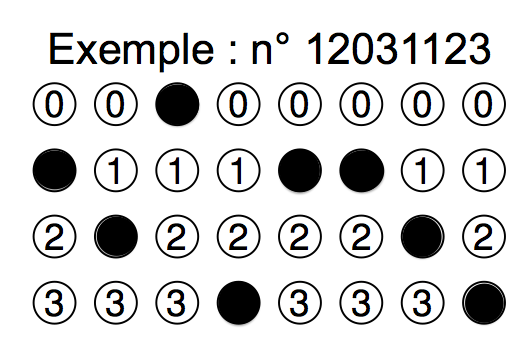
\includegraphics[trim = 30px 0 0 77px, clip,scale=0.25]{src/graphics/expleNoEtudiant.png}\hspace*{\fill}

\AMCcode{etu}{8}\hspace*{\fill}
\begin{minipage}[b]{6.5cm}\setlength{\parindent}{0pt}
$\longleftarrow{}$\hspace{0pt plus 1cm} encodez votre numéro d'étu\-diant ci-contre,
et inscrivez votre nom, prénom et numéro de place ci-dessous.

\vspace{3ex}

\hfill\champnom{\fbox{
    \begin{minipage}{.9\linewidth}
      Nom:

      \vspace*{.5cm}\dotfill

      Prénom:

      \vspace*{.5cm}\dotfill

      Place:

      \vspace*{.5cm}\dotfill

      \vspace*{1mm}
    \end{minipage}
  }}\hfill\vspace{5ex}

\end{minipage}\hspace*{\fill}

}

\vspace{5ex}

{\bf\em\setlength{\parindent}{0pt} Les réponses aux questions sont à donner exclusivement sur cette feuille :
  les réponses données sur d'autres feuilles ne seront pas prises en compte.

\vspace{1ex}
Coloriez complètement et proprement chaque case choisie, afin d'obtenir le meilleur contraste possible
par rapport à une case vide. Ne coloriez pas les cases au crayon à papier, n'utilisez pas de
couleur rouge (le programme correcteur ne voit pas les couleurs). Utilisez plutôt du noir ou du bleu foncé.
Pour corriger une éventuelle erreur de saisie, veuillez utiliser si possible un correcteur liquide (Tipp-Ex).
}

\vspace{2ex}

%%% fin de l'en-tête de la feuille de réponses

\begin{multicols}{2}
\setlength{\parindent}{0pt}
\formulaire
\end{multicols}

\clearpage

}

\end{document}